\documentclass{beamer}
\usetheme{Warsaw}
\title{Turing Machine Project Introduction}
\author{Chad Spensky \\
        Stuart Baker \\
        Tim Greer\\
        Jack Lepird}
\begin{document}
\maketitle

\begin{frame}
\frametitle{Overview}
\begin{itemize}
\item Introductions
\item What is a Turing Machine?
\item Agenda for Today
\end{itemize}

\end{frame}

\section{Introductions}


% Should be able to just copy and paste to create your own slide
\subsection{Jack Lepird}
\begin{frame}
\frametitle{Jack Lepird}
\begin{columns}
\column{0.5\textwidth} % Info column 
\begin{itemize}
\item Background: Machine Learning, Optimization, and Artificial Intelligence
\item Research: Next-Generation Aircraft Collision Avoidance Systems
\item Hobbies: Travel, SCUBA, Golf
\end{itemize}

\column{0.5\textwidth} % Picture column
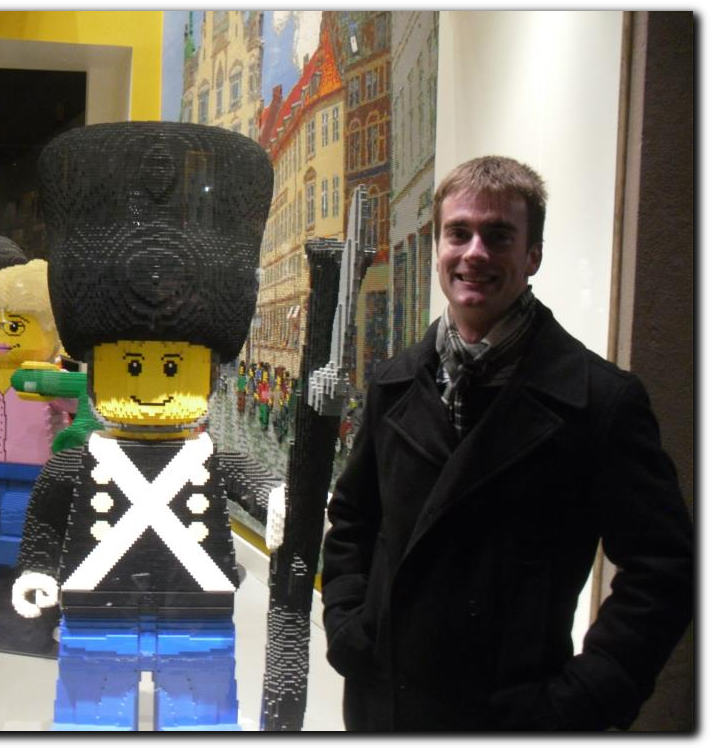
\includegraphics[width=5cm]{jack.png}
\end{columns}
\end{frame}

\subsection{You?}
\begin{frame}
And you?
\end{frame}

\section{What is a Turing Machine}

\section{Agenda for Today}

\end{document}


